\section{FreMEn - Predicting Future Occupancy}
\label{sec:fremen}
The  Frequency Map Enhancement (FreMEn) method models the dynamics of each cell by its primary frequency components. 
It has successfully been applied to improve mobile robots ability to perform feature-based localization \cite{online_fremen} and topological navigation \cite{fentanes2015}. 
Here Krajník et al. argues for approximating the appearance and disappearance of obstacles with multiple periodic sinus signals, since people often moves them as part of daily routines. 
As discussed in section \ref{sec:characteristics_in_industrial_environments} this might also be the case in the industrial environments in focus here. 

Resent work in \cite{life_long_exploration}, shows how the often violated assumption in FFT about a fixed sampling rate is met by incrementally adding sparse and irregular observations. 
This will probably decrease the prediction performance, but enables online updates without having to store observations for evaluation. 
Where this approach usually uses the number of frequency components that minimizes the difference between predicted states and measurements, it is chosen to always use the typical order of three \cite{life_long_exploration} for all cells.

\subsection{Online Learning of Frequency Components}
The online variant of the FreMEn method updates the parameters shown in equation \ref{eq:fremen_update} for each  observed probability for occupancy $p(t)$. 

\begin{eqnarray}
\alpha_0 &=& \frac{1}{n+1}(n \alpha_0 + p(t)) \nonumber \\ 
\gamma_k &=& \frac{1}{n+1}(n \gamma_k + p(t) e^{-j \omega_k t}) \forall \omega_k \in \Omega  \\
\beta_k &=& \frac{1}{n+1}(n \beta_k + \alpha_0 e^{-j \omega_k t}) \forall \omega_k \in \Omega \nonumber \\
n &=& n + 1 \nonumber
\label{eq:fremen_update}
\end{eqnarray}

The average occupancy probability $\alpha_0$ models the $0Hz$ signal and is updated with a new measurement online, and the number of measurements $n$ is incremented. 
For each of the frequency components $\omega_k=1/T_k$ there are the complex numbers; $\gamma_k$ and $\beta_k$.
$T$ is calculated with equation \ref{eq:fremen_time} for each frequency, where $N$ is the $20$ used frequency components and epsilon is the smallest time period, which is $100$ seconds here. 
The values of consecutive $T_k$ is close for large values of $k$, which is advantageous if most of the obstacles moves with a period close to $\epsilon$.

\begin{equation}
T_k = \frac{N \epsilon}{k+1}
\label{eq:fremen_time}
\end{equation}

The real and imaginary part of $\gamma_k$ and $\beta_k$ are updated as the running average. $\gamma_k$ is the part of the signal with the frequency $2 \pi \omega_k$, and $\beta_k$ is the part of this signal which are modeled by the $0Hz$ component of the signal.

When predicting the state of a cell at time $t$ the signal components are calculated with equation \ref{eq:fremen_freq_component}.
Then $ \Omega $ is ordered based on $ \left\| \alpha_k \right\| $ to enable calculation of equation \ref{eq:fremen_predict} using only the $m=order-1=2$ most prominent frequency components.
The function $\zeta$ clamps the expected signal to one if it is above $0.5$ and zero else. The $arg$-function returns the angle of the complex number with respect to the real axis.
The occupancy state at time $t$ is predicted as occupied if $s(t)$ is one and as free if it is zero.

\begin{equation}
\alpha_k = \gamma_k - \beta_k \forall \omega_k \in \Omega
\label{eq:fremen_freq_component}
\end{equation}

\begin{equation}
s(t) = \zeta \left( \alpha_0 \sum_{k=1}^{m} |\alpha_k| cos(\omega_k t + arg(\alpha_k))  \right)
\label{eq:fremen_predict}
\end{equation}

\subsection{Evaluation in a Simulated Dynamic Environment}
The methods ability to predict future occupancy states are evaluated in a Stage simulation \cite{Vaughan2008} where many boxes moves in and out at various fixed intervals. 
The robot continuously navigates from the lower left corner that are partly surrounded by walls to the top right corner, while green boxes moves around.

\begin{figure}[htbp]
    \centering
    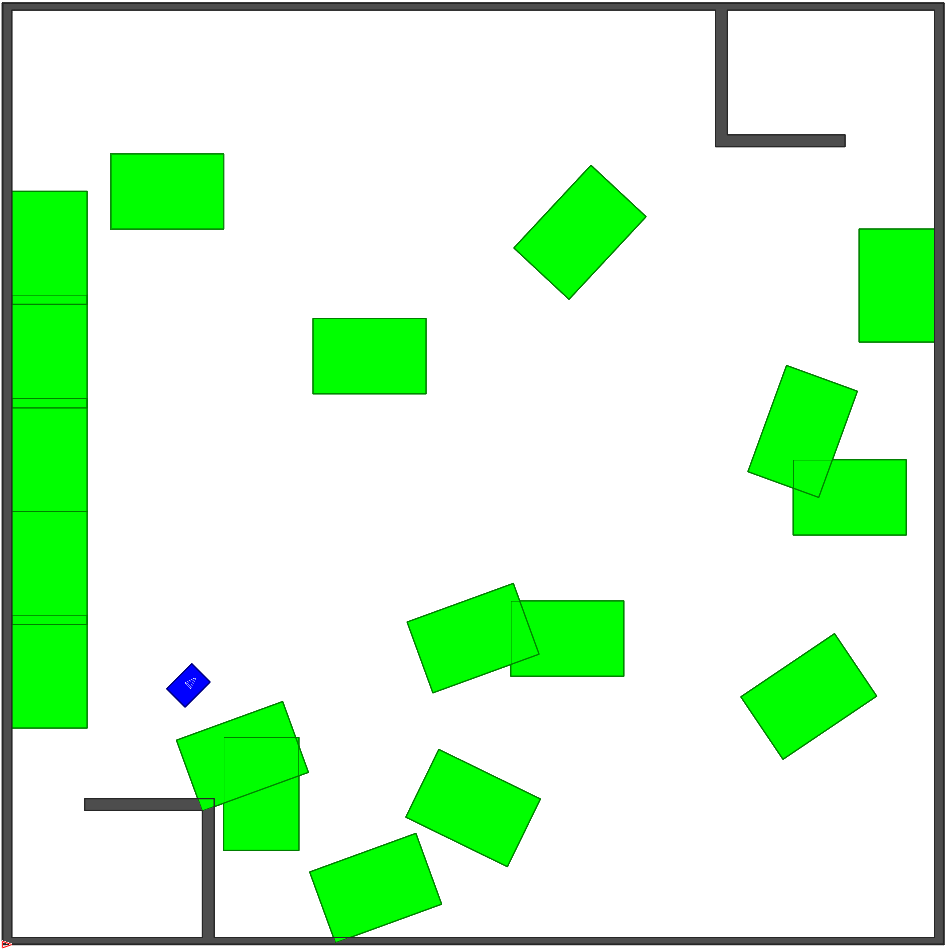
\includegraphics[width=0.4\linewidth]{chapters/mapping_of_dynamic_areas/figures/simulated_environment}
    \caption{Screen shot of the Stage simulator showing a MiR-100 robot navigating around obstacles which appears and disappears at fixed intervals.}
    \label{fig:simulated_environment}
\end{figure}

The static mapper incorporates the measurements from the simulated LIDARs into a temporary local map. 
For every fifth second a global map of FreMEn cells are updated with \ref{eq:fremen_update} where $p(t)$ is the probability for occupancy in the local map. 
The local map is then cleared and the process continues.

\subsection{Predictive Capabilities}
To evaluate the predictive strength of FreMEn it is used to predict the appearance of obstacles each time a new measurement is added from the local map. 
Figure \ref{fig:fremen_ideal_sim} shows how FreMEn correctly predicts the appearance of many of the obstacles when the robots exact position is used to incorporate exact LIDAR measurements. 

\begin{figure}[htbp]
    \centering
    \begin{subfigure}[t]{0.49\textwidth}
        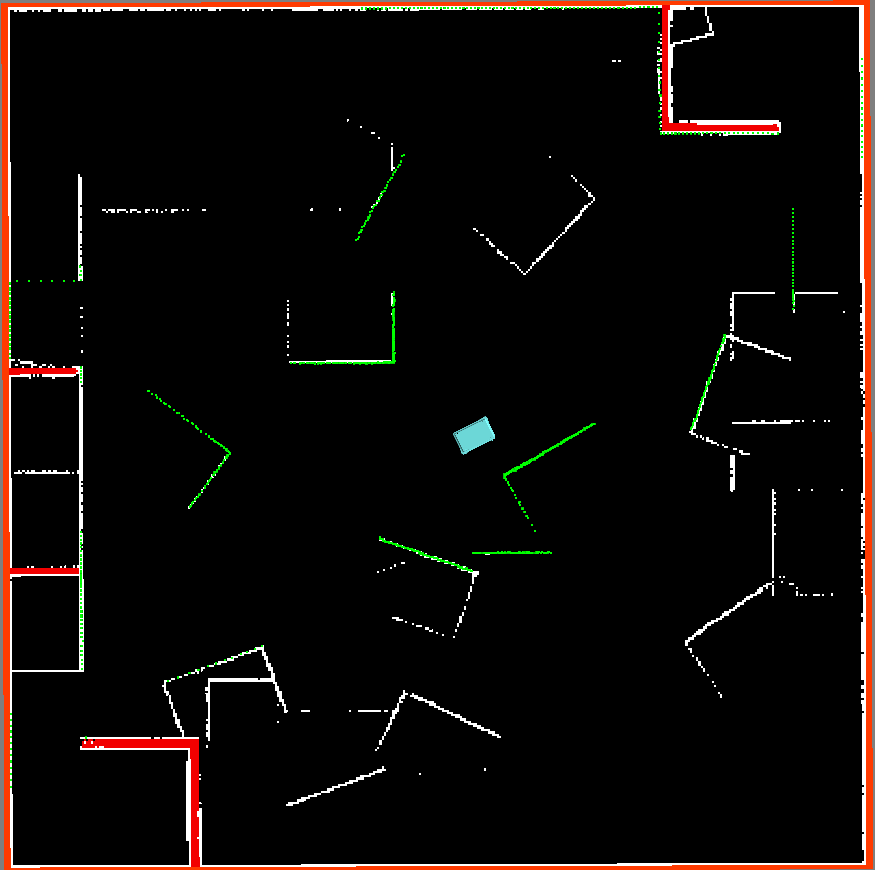
\includegraphics[width=1.0\textwidth]{chapters/mapping_of_dynamic_areas/figures/fremen_ideal_simulation}	
        \caption{Predicted map without noise.}
        \label{fig:fremen_ideal_sim}
    \end{subfigure}
    \begin{subfigure}[t]{0.49\textwidth}
        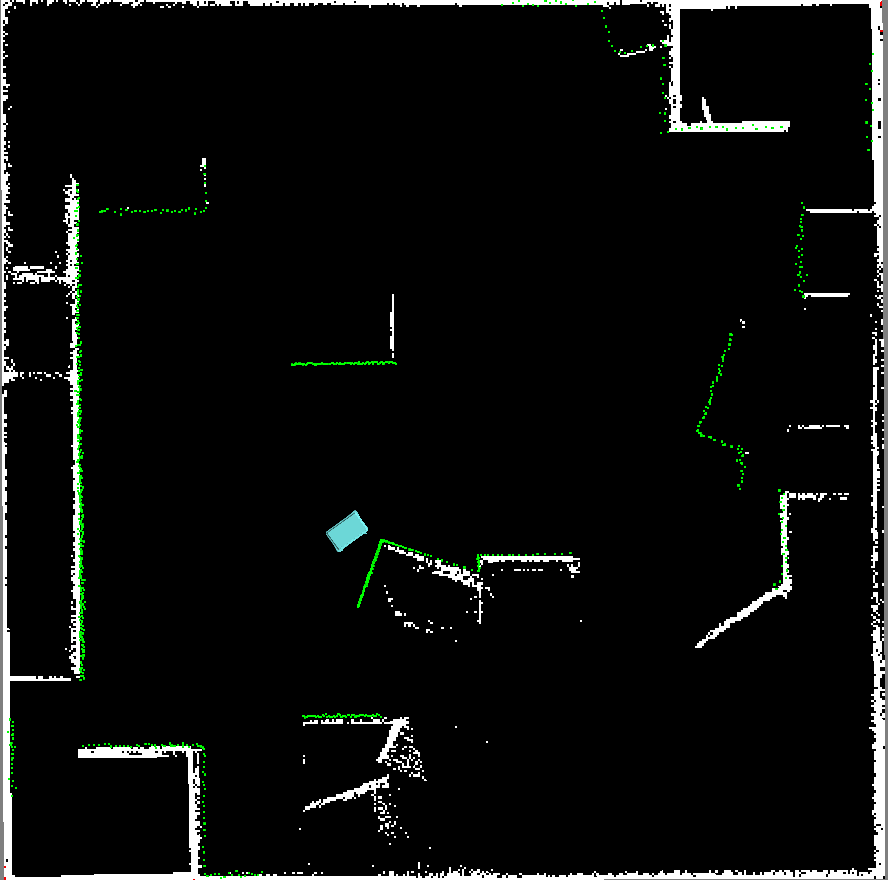
\includegraphics[width=1.0\textwidth]{chapters/mapping_of_dynamic_areas/figures/fremen_with_decay_last}
        \caption{Predicted map with realistic sensor and localization noise.}
        \label{fig:fremen_sim_with_noise}
    \end{subfigure}
    \caption{Robot navigating on the map predicted with FreMEn where the the green dots marks ends of LIDAR readings. The colors; Black, red and white, represents free, unknown and obstacle.}
\end{figure}

Figure \ref{fig:fremen_avg_miss_with_noise} shows a more realistic simulation with Gaussian noise on LIDAR measurements with a standard deviation of one centimeter, and localization using AMCL with a static map representation of the black walls in figure \ref{fig:simulated_environment}.
Here some of the obstacles are predicted to have moved while they in fact are still present, as shown in the middle to the right in figure \ref{fig:fremen_avg_miss_with_noise}.

FreMEn's lack of ability to predict future measured obstacles is also apparent in the average correctly predicted observations of obstacles. This measure is calculated with equation \ref{eq:average_predict_score}, where $s$ is the state that can be; occupied or free, and $n_{cells}$ is the number of cells that are either observed or predicted as occupied.

\begin{equation}
\text{Average correct obstacle prediction} = \left[1- \frac{\sum\limits_{i=1}^{n_{cells}} \left\|s_{predict}(i)-s_{observation}(i)\right\|}{n_{cells}}
\right]\cdot 100
\label{eq:average_predict_score}
\end{equation} 

This is shown in figure \ref{fig:fremen_avg_correct_predictions} where the good prediction percentage of $74.0\%$ drops to $46.9\%$ with the addition of noise.
From the experiment without noise it is concluded that the learned periodic appearance of obstacles in a grid with FreMEn is useful for predictions.
In the presence of noise the signals within the cells becomes more complicated, and the measurements used for comparison is not always correct.
This, combined with the fact that obstacles placed by humans will probably not move in and out of grid cells so consistently as in this simulation, leads us to believe that the implemented method is not optimal for online updates of occupancy grid maps used by AMCL.
It might however be possible to alter the method, or combine it with others, to take advantage of the methods ability to predict presence of obstacles many hours after the last observation.
The predicted maps can improve the validity of global paths planned by the robot, but with the rather poor prediction percentage many paths have to be re-planned during navigation.

\begin{figure}[htbp]
    \centering
    \begin{subfigure}[t]{0.49\textwidth}
        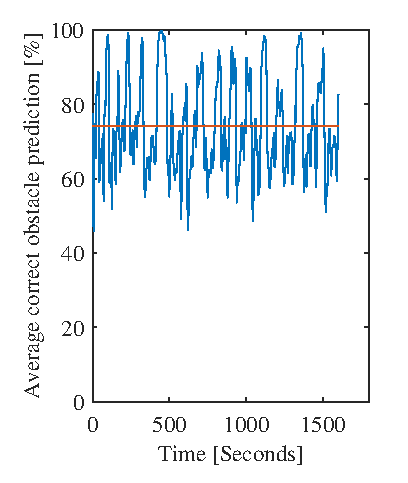
\includegraphics[width=1.0\textwidth]{chapters/mapping_of_dynamic_areas/figures/fremen_avg_miss_no_noise}	
        \caption{Prediction score without noise.}
        \label{fig:fremen_avg_miss_no_noise}
    \end{subfigure}
    \begin{subfigure}[t]{0.49\textwidth}
        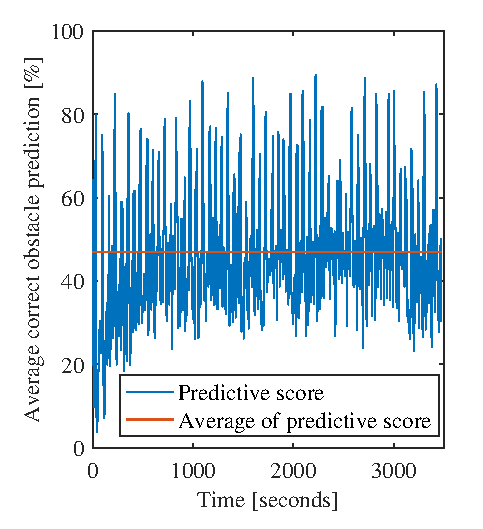
\includegraphics[width=1.0\textwidth]{chapters/mapping_of_dynamic_areas/figures/fremen_avg_miss_with_noise}
        \caption{Prediction score with noise.}
        \label{fig:fremen_avg_miss_with_noise}
    \end{subfigure}
    \caption{Prediction scores for FreMEn defined as the average number of matches between measured and predicted obstacles.}
    \label{fig:fremen_avg_correct_predictions}
\end{figure}